\documentclass[conference]{IEEEtran}
\IEEEoverridecommandlockouts
% The preceding line is only needed to identify funding in the first footnote. If that is unneeded, please comment it out.
\usepackage{cite}
\usepackage{amsmath,amssymb,amsfonts}
\usepackage{algorithmic}
\usepackage{graphicx}
\usepackage{textcomp}
\usepackage{xcolor}
\def\BibTeX{{\rm B\kern-.05em{\sc i\kern-.025em b}\kern-.08em
    T\kern-.1667em\lower.7ex\hbox{E}\kern-.125emX}}
\begin{document}
% \title{Navigator For Visually Impaired Person\\
% % {\footnotesize \textsuperscript{*}Note: Sub-titles are not captured in Xplore and
% % should not be used}
% % \thanks{Identify applicable funding agency here. If none, delete this.}
% }

% \author{\IEEEauthorblockN{1\textsuperscript{st} Swati Patil}
% \IEEEauthorblockA{\textit{Dept. of Electronics and Telecommunication} \\
% \textit{name of organization (of Aff.)}\\
% City, Country \\
% email address or ORCID}
% \and
% \IEEEauthorblockN{2\textsuperscript{nd} Given Name Surname}
% \IEEEauthorblockA{\textit{Dept. of Electronics and Telecommunication} \\
% \textit{name of organization (of Aff.)}\\
% City, Country \\
% email address or ORCID}
% \and
% \IEEEauthorblockN{3\textsuperscript{rd} Given Name Surname}
% \IEEEauthorblockA{\textit{Dept. of Electronics and Telecommunication} \\
% \textit{name of organization (of Aff.)}\\
% City, Country \\
% email address or ORCID}
% \and
% \IEEEauthorblockN{\hspace{2.65cm}4\textsuperscript{th} Given Name Surname}
% \IEEEauthorblockA{\hspace{2.50cm}\textit{dept. name of organization (of Aff.)} \\
% \textit{\hspace{2.50cm}name of organization (of Aff.)}\\
% \hspace{2.50cm}City, Country \\
% \hspace{2.50cm}email address or ORCID}
% \and
% \IEEEauthorblockN{5\textsuperscript{th} Given Name Surname}
% \IEEEauthorblockA{\textit{dept. name of organization (of Aff.)} \\
% \textit{name of organization (of Aff.)}\\
% City, Country \\
% email address or ORCID}
% }

\title{Navigator For Visually Impaired Person\\
% {\footnotesize \textsuperscript{*}Note: Sub-titles are not captured in Xplore and
% should not be used}
% \thanks{Identify applicable funding agency here. If none, delete this.}
}

% \author{Swati Patil, Nikhil Kanitkar, Dewoo Kudtarkar, Mandar Naik, Pranit Patil\\
% \textit{Department of Electronics and Telecommunication Engineering\\ Bharati Vidyapeeth College of Engineering\\\normalfont Belpada, Navi Mumbai, Maharashtra, India.\\swati.patil@bvcoenm.edu.in, nikhil\_k23@pm.me, dewoo\_k@pm.me, MDnaik@pm.me, pranit\_p48@pm.me}
% }

% \author{\textbf{Swati Patil\textsuperscript{1}, Nikhil Kanitkar\textsuperscript{2}, Dewoo Kudtarkar\textsuperscript{3}, Mandar Naik\textsuperscript{4}, Pranit Patil\textsuperscript{5}\vspace{0.5cm}}\\
% \textit{1,2,3,4,5 Department of Electronics and Telecommunication Engineering, Bharati Vidyapeeth\\College of Engineering, Belpada, Navi Mumbai, Maharashtra, India\vspace{0.5cm}}
% }

\makeatletter
\newcommand{\newlineauthors}{%
  \end{@IEEEauthorhalign}\hfill\mbox{}\par
  \mbox{}\hfill\begin{@IEEEauthorhalign}
}
\makeatother

\author{\IEEEauthorblockN{Swati Patil,}
\IEEEauthorblockA{\textit{Department of EXTC},\\
\textit{Bharati Vidyapeeth} \\ \textit{College of Engineering},\\
Navi Mumbai, India.\\
swati.patil@bvcoenm.edu.in}
\and
\IEEEauthorblockN{Nikhil Kanitkar,}
\IEEEauthorblockA{\textit{Department of EXTC},\\
\textit{Bharati Vidyapeeth} \\ \textit{College of Engineering},\\
Navi Mumbai, India.\\
nikhilkanitkar1301@gmail.com}
\and
\IEEEauthorblockN{Dewoo Kudtarkar,}
\IEEEauthorblockA{\textit{Department of EXTC},\\
\textit{Bharati Vidyapeeth} \\ \textit{College of Engineering},\\
Navi Mumbai, India.\\
dewookudtarkar@gmail.com}
\newlineauthors
\IEEEauthorblockN{Mandar Naik,}
\IEEEauthorblockA{\textit{Department of EXTC},\\
\textit{Bharati Vidyapeeth} \\ \textit{College of Engineering},\\
Navi Mumbai, India.\\
mandarnaik016@gmail.com}
\and
\IEEEauthorblockN{Pranit Patil,
}
\IEEEauthorblockA{\textit{Department of EXTC},\\
\textit{Bharati Vidyapeeth} \\ \textit{College of Engineering},\\
Navi Mumbai, India.\\
pranitpatil02244@gmail.com}
}

\maketitle

\begin{abstract}
A device called a navigator for visually impaired persons uses auditory commands to aid or direct people who are blind or have vision loss, ranging from partial sight. The proposed system will be suitable for reducing collision risks by enabling an impaired person to walk outdoors easily. A visually impaired person can take outputs via voice assistants and sensors. The suggested result includes a camera-based vision system to make an independent operation for out-of-door navigation using the latest technology and create a good user experience for blind people. The system will collect information about objects and the distance between them. The system is designed to detect all objects in front of the person. The development of the smart navigator must be affordable so that in the commercial market, it is helpful for a visually impaired person.
\end{abstract}

\begin{IEEEkeywords}
navigator system, visually impaired, voice assistant, smart device
\end{IEEEkeywords}

\section{INTRODUCTION}
Around 12 million Indians are visually impaired due to untreated refractive error, according to the WHO. Many visually impaired persons come from deprived backgrounds and reside in tier 4 cities and rural areas without access to spectacles. However, they need to be made aware that this is curable. Visually impaired people use canes for their daily tasks, but walking on the road and dealing with their daily tasks is not easy. It affects their freedom and threatens them with many everyday tasks, with the focus being placed on those that involve moving through a strange environment. 

Multiple devices are present in our society to overcome the problems of visually impaired people. Specific models are available in the market, but they cannot handle visually impaired people. A smart cap is not capable of recognizing objects near that person. Some devices are based on internet connectivity; hence, they are unreliable. Smart eye device is difficult to detect objects at ground level. 

Smart sticks cannot detect hidden obstructions, which are very dangerous for the blind person, such as under stairs and holes. Identifying all those difficulties, we build a model that identifies ground and objects at the eye-sight level. 

This navigation system is designed to help blind people to navigate around safely. To detect the obstacle, the user need not be required to move the white cane around. As a result, a person can go around without using a cane and continuously hear from speakers about potential hazards.

% Our model can operate model without internet connectivity as well. Easy to carry anywhere in Environment. Long life battery and Simple system to operate. Many Devices are more Costier and not affordable to tier 2 and 3 cities. Our model is Affordable and Sustainable for those people.

\section{LITREATURE REVIEW}
Recent studies on global health estimate that millions of people have a visual impairment. Based on the research, many papers introduce improvement technology on the smart cane. In advance, the way researchers are trying to transplant real eyes with the help of robotic eyes. 

Many research papers are based on smart caps, smart assistive, and smart eyes. [1] uses TensorFlow API for object detection in that OpenCV helps in the image operations. Those systems are unable to recognize objects near that person. Whereas [2] is based on smart glass, which is based on internet connectivity; hence, it is unreliable. 

The solution in [3] is based on a voice-enabled system that would direct messages to visually challenged people in their daily tasks. In [4], They provided a solution for blind individuals by incorporating an ultrasonic sensor into the blind stick. However, they could not identify hazards for the blind, such as holes and descending steps. In [5] ultrasonic system detects objects in front of the person, and then its output gives to the vibration sensor. 

The [6] is an IoT-based device with an ultrasonic sensor. In this user need to connect to Bluetooth at all time for the last location of the person. In the indoor navigation system, a wearable travel aids system is mounted on the head. The ultrasonic sensor is inserted in the mounted head system. It detects hanging obstacles; its output comes from audio and tactile displays. 

The [7] system uses GPRS-based devices to reach the user's destinations. In this device, the user's destination request goes to the server device and finds the shortest distance between the user and the destination. The [8] system is based on a camera module that raspberry pi uses as an image processor, and the output comes in the form of audio. 

% \subsection{Maintaining the Integrity of the Specifications}

% The IEEEtran class file is used to format your paper and style the text. All margins, 
% column widths, line spaces, and text fonts are prescribed; please do not 
% alter them. You may note peculiarities. For example, the head margin
% measures proportionately more than is customary. This measurement 
% and others are deliberate, using specifications that anticipate your paper 
% as one part of the entire proceedings, and not as an independent document. 
% Please do not revise any of the current designations.

\section{METHODOLOGY}
The solution proposed can be divided into two parts, that is one for the upper half and another for the lower half of the body. The upper half is responsible for object detection along with their distance using smart glasses, whereas the lower half takes care of obstacles near to legs using smart shoes.

\begin{figure}[h]
\centering
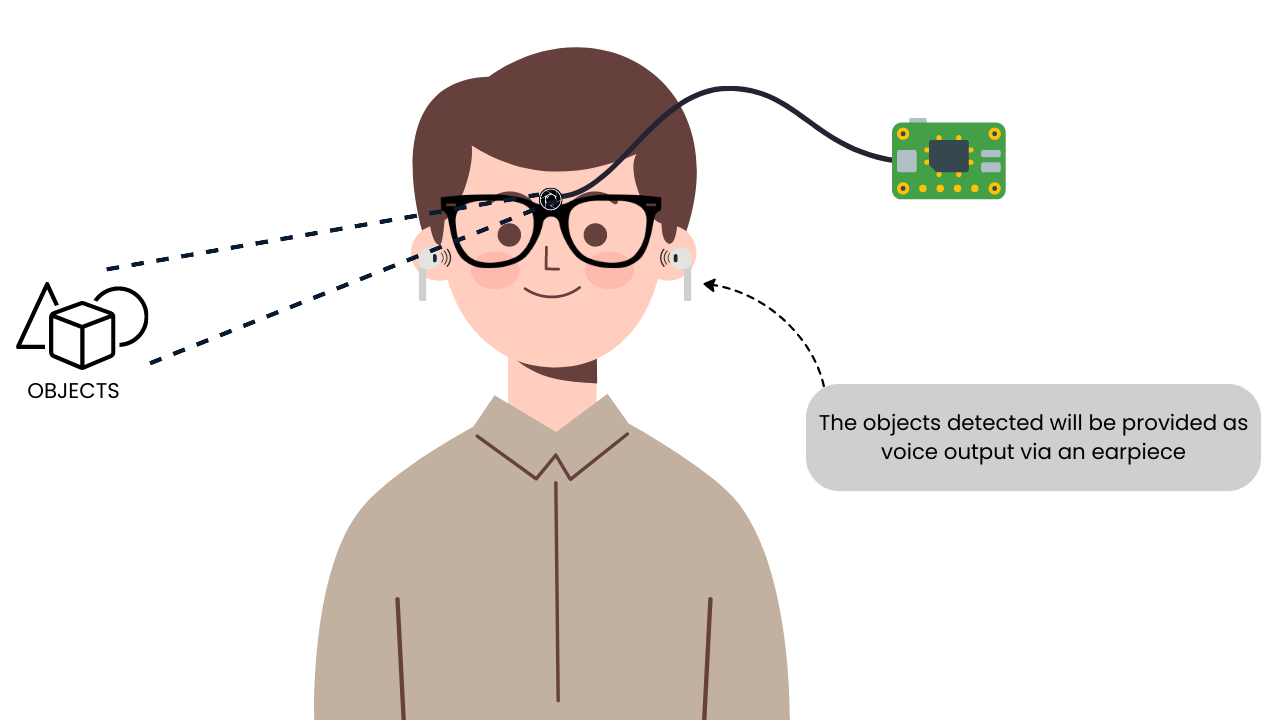
\includegraphics[width=3in\textwidth]{graphic_upper_300_DPI.png}
\caption{Smart glasses.}
\label{fig_sim}
\end{figure}

As illustrated, smart glasses will capture the objects and will notify the impaired user regarding the detected objects via an earpiece. 

\begin{figure}[h]
\centering
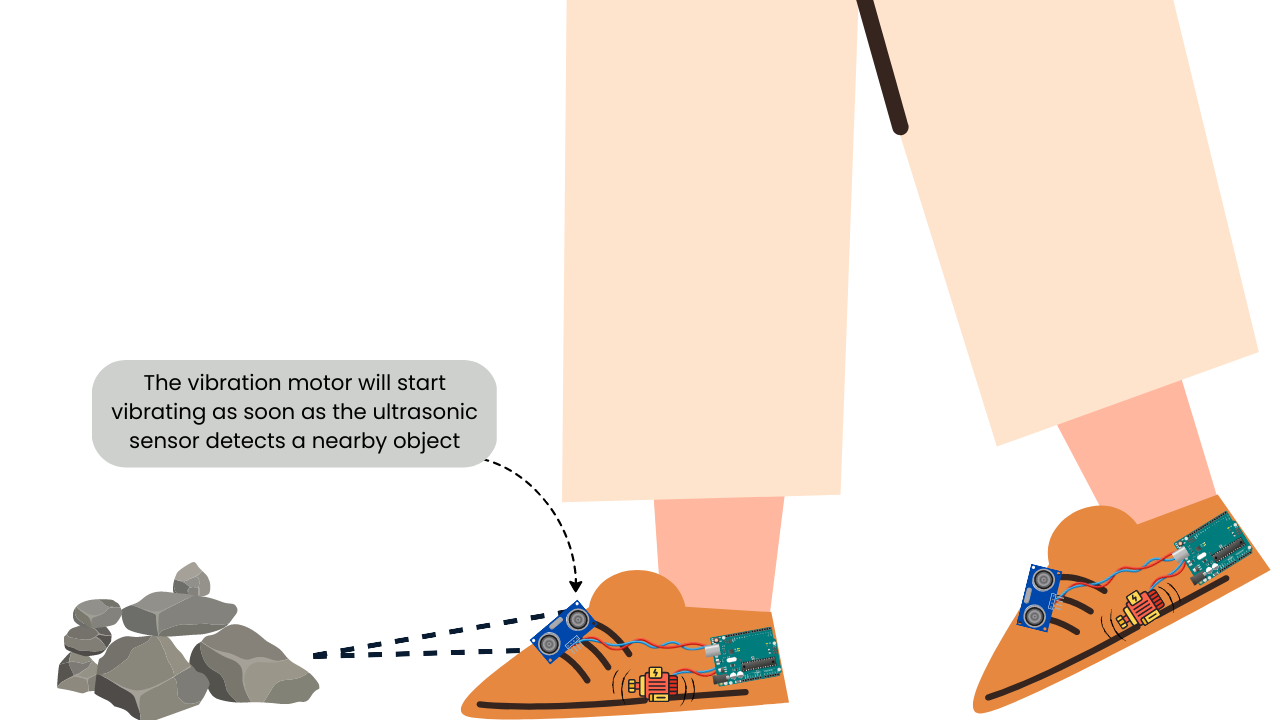
\includegraphics[width=3in\textwidth]{graphic_lower_300_DPI.png}
\caption{Smart shoes.}
\label{fig_sim}
\end{figure}

At the same time, smart shoes will constantly check for obstacles. They will notify them via a vibration produced by a vibration motor whenever the obstacle is in a specific range from the sensor.

\subsection{Block Diagram}

Obstacles in our environment are referred to as objects. Obstacles are captured using the Pi camera, a Raspberry Pi camera. Raspberry Pi serves as a computer's processing unit. YOLO is used to find and identify objects. It also determine the distance using reference photos. An earpiece is a device that outputs voice signals.

\begin{figure}[h]
\centering
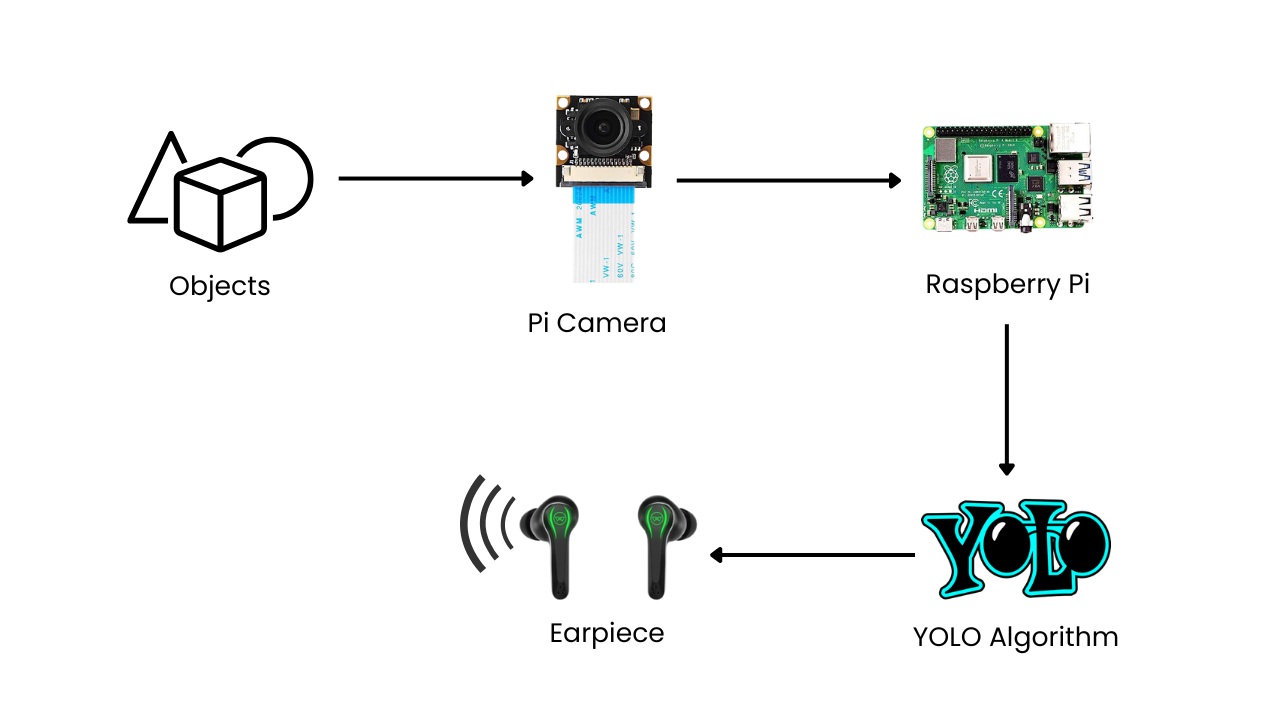
\includegraphics[width=3.7in\textwidth, height=2.2in]{block_upper_300_DPI.png}
\caption{Block diagram for smart glasses.}
\label{fig_sim}
\end{figure}

 The ultrasonic sensor measures the separation between people and objects. The Arduino nano is also a processing tool used to process data from an ultrasonic sensor. A vibration motor alerts a person when an obstruction is within a predetermined distance. 
 
\begin{figure}[h]
\centering
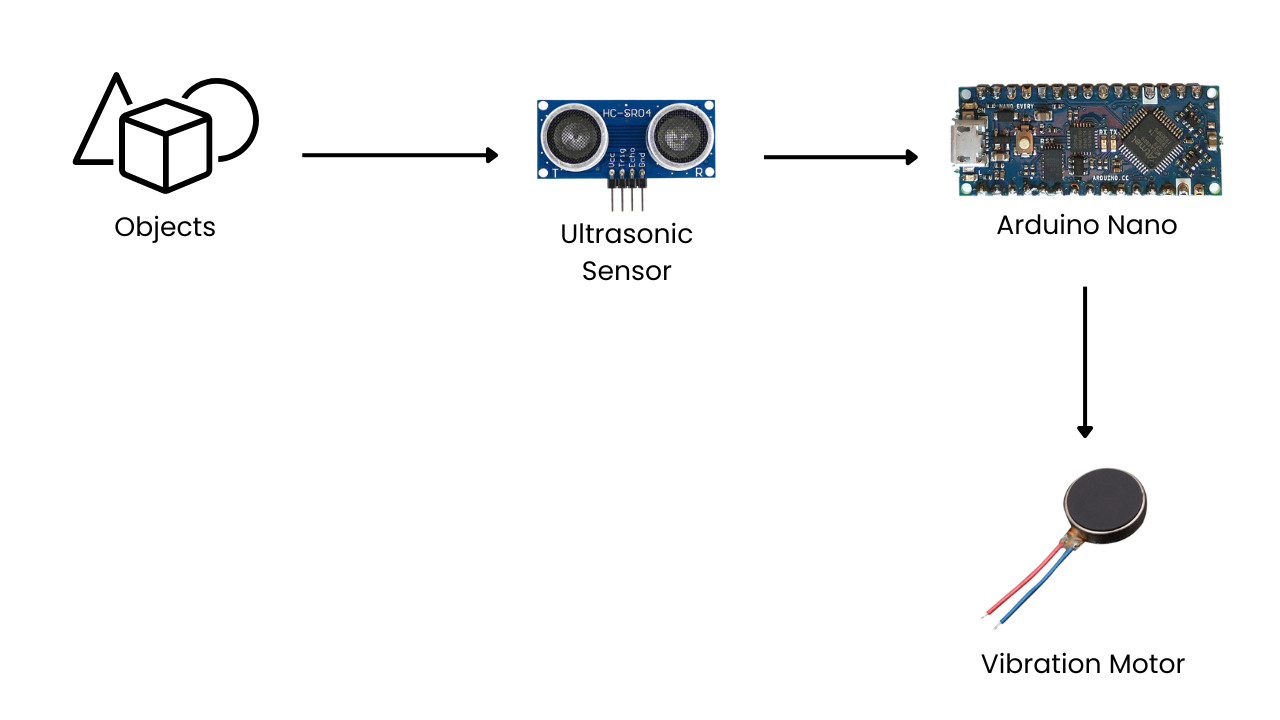
\includegraphics[width=3.3in\textwidth, height=2.2in]{block_lower_300_DPI.png}
\caption{Block diagram for smart shoes.}
\label{fig_sim}
\end{figure}

\subsection{Flowchart}

\begin{figure}[h]
\centering
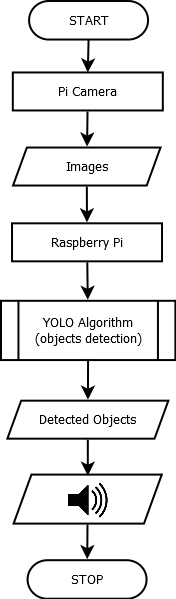
\includegraphics[width=1.4in\textwidth, height=3.6in]{flowchart_upper_300_DPI.png}
\caption{Flowchart for smart glasses.}
\label{fig_sim}
\end{figure}

Figure 5 shows a flowchart on how the smart glasses operate. After turning on the device, the camera will start capturing images of the surroundings. It will pass them as output to raspberry pi, using the YOLO algorithm to detect and identify objects along with their distance. This output of raspberry pi will be notified to the visually impaired person via an earpiece in audio form.

Figure 6 shows a flowchart on how the smart shoes operate. The smart shoe is a technologically advanced footwear designed for the modern, tech-savvy individual. Equipped with an ultrasonic sensor, Arduino nano, and vibration motor, it combines fashion and functionality in one package.

The shoe's ultrasonic sensor enables it to recognize threats and obstructions in real time, giving the wearer an added security measure as they navigate their surroundings. The smart shoe's key component is an Arduino nano, which enables it to interface with other gadgets and use a vibration motor to give the wearer real-time input. For instance, when the ultrasonic sensor detects an obstruction in front of the wearer, the vibration motor will start up to inform the user so they can take evasive action.

\begin{figure}[h]
\centering
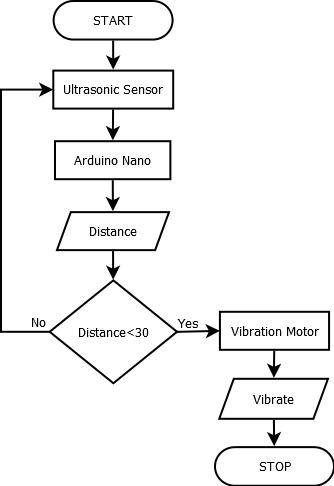
\includegraphics[width=2.4in\textwidth, height=3.6in]{flowchart_lower_300_DPI.png}
\caption{Flowchart for smart shoes.}
\label{fig_sim}
\end{figure}

\subsection{Algorithm and framework}
The YOLO framework deals with object detection in a novel way. It predicts these boxes bounding box coordinates and class probabilities using the complete image in a single instance. 

\begin{figure}[h]
\centering

\includegraphics[width=2in\textwidth]{YOLO_300_DPI.png}
\caption{YOLO algorithm.}
\label{fig_sim}
\end{figure}

We have used the YOLO algorithm and distance estimation code based on the focal length concept. We used the reference images of each object and provided the distance for that object from the camera lens. While processing for each frame detected object distance is estimated using the image pixels' position. 

We wrote the function for the focal length finder. In this code, we integrated the text-to-speech block of code. Put that code in a loop to extract the output in the form of voice. The most significant advantage of using YOLO is its fast processing speed (45 frames per second). Additionally, YOLO is aware of generic object representation. 

The YOLO algorithm advantage is as follows:
\begin{enumerate}[\IEEEsetlabelwidth{12)}]
\item Speed: Because this algorithm can forecast real-time
objects, it increases the detection speed.
\item High accuracy: The YOLO prediction method produces
exact results with low errors in the background.
\item Due to its superior learning capabilities, the algorithm can learn and use the representations of things in object detection.
\end{enumerate}

\section{RESULT}

The Picamera module is mounted on the glasses to detect the object from the eye-sighting level. 

\begin{figure}[h]
\centering
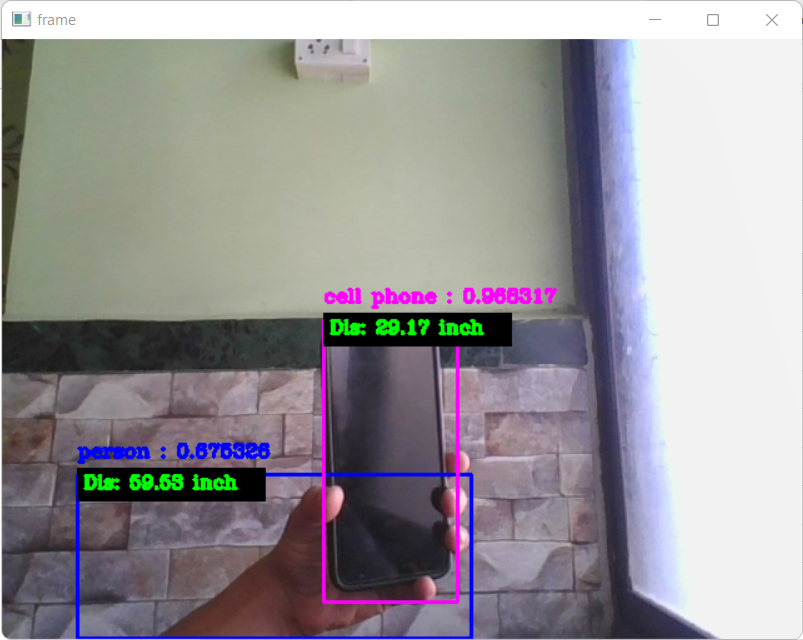
\includegraphics[width=2.5in\textwidth]{2023-02-12 14_13_19-frame_300_DPI.png}
\caption{Detection and Identification of mobile phone}
\label{fig_sim}
\end{figure}

The camera captures the real-time video and processes it frame by frame to give the output that is detected object and that object estimate distance from the camera. It is done by the technique which uses the focal length concept. The output is retrieved from the Bluetooth-enabled earphone device after processing.

\begin{figure}[h]
\centering
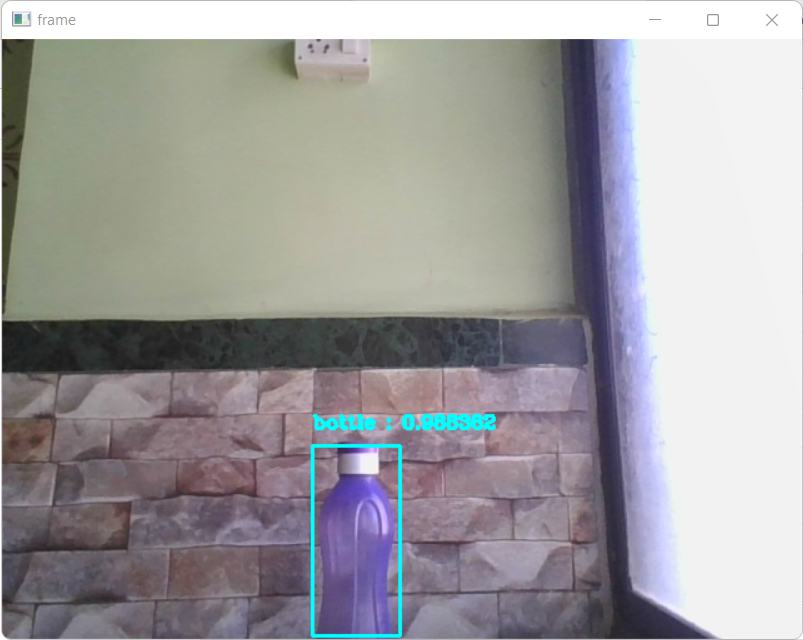
\includegraphics[width=2.5in\textwidth]{2023-02-12 14_11_37-frame_300_DPI.png}
\caption{Detection and Identification of Bottle}
\label{fig_sim}
\end{figure}

Multiple objects of the same type may also be found and recognized. These detected objects will then be provided as output via earpiece.

% \begin{figure}[h]
% \centering
% 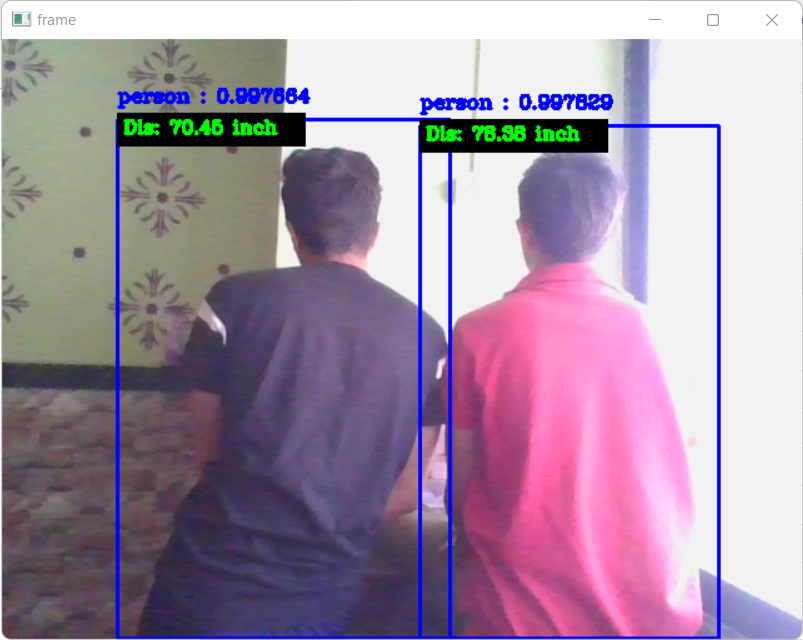
\includegraphics[width=2.5in\textwidth]{2023-02-12 14_16_20-frame_300_DPI.png}
% \caption{Detection and Identification of Persons}
% \label{fig_sim}
% \end{figure}

\begin{figure}[h]
\centering
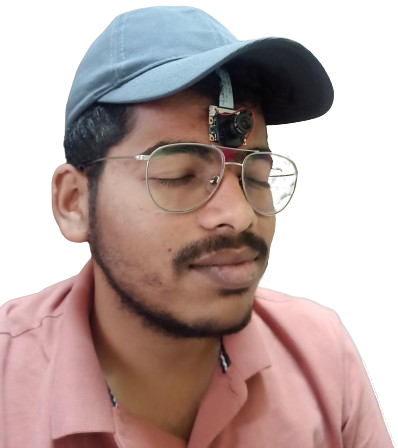
\includegraphics[width=2.5in\textwidth]{Glasses_300_DPI.png}
\caption{Smart glasses prototype}
\label{fig_sim}
\end{figure}

\begin{figure}[h]
\centering
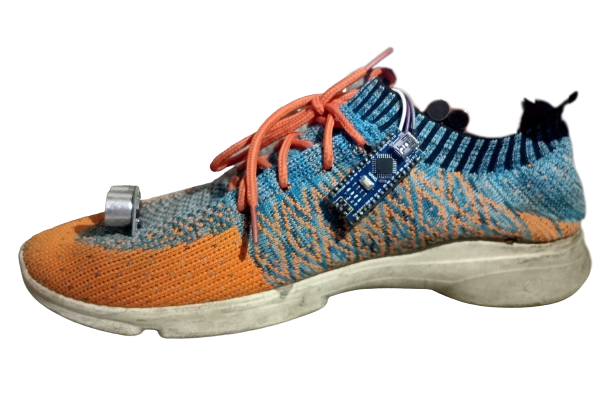
\includegraphics[width=2.5in\textwidth]{prototype_shoe_300_DPI.png}
\caption{Smart shoes prototype}
\label{fig_sim}
\end{figure}

The ultrasonic sensor detects objects near the foot with a cutoff distance of 30 cm less than that distance. The object gets detected, and a response is provided to the person with the help of vibrating motors with mild vibrations so that the person can easily recognize it and change the direction of walking accordingly.

\section{CONCLUSION}

Visually impaired people face many problems in their daily life. While travelling, they always depend on any person or guide dog. The blind stick is very helpful for them, but the stick has certain restrictions. This project is to make their task easy and simple. The navigator system aims to make it affordable and safe to use. The person who uses it does not require any particular skill to operate this system. Our system is helpful and can aid every visually impaired individual. We can increase the number of objects in this system as per user needs.

% \section*{Acknowledgment}
% The preferred spelling of the word ``acknowledgment'' in America is without 
% an ``e'' after the ``g''. Avoid the stilted expression ``one of us (R. B. 
% G.) thanks $\ldots$''. Instead, try ``R. B. G. thanks$\ldots$''. Put sponsor 
% acknowledgments in the unnumbered footnote on the first page.

\begin{thebibliography}{00}
\bibitem{b1}  Nishajith. A, Nivedha. J, Shilpa.S.Nair, Prof.Mohammed Shaffi. J, “Review paper on - Smart Cap-Wearable Visual Guidance System For Blind”, Proceedings of the International Conference on Inventive Research in Computing Applications (ICIRCA), pp. 275-277, 2018.
\bibitem{b2}  Arjun Pardasani, Prithviraj N Indi, Sashwata Banerjee, Aditya Kamal, “Review paper on-Smart Assistive Navigation Devices for Visually Impaired People”, International Conference on Computer and Communication Systems, pp. 725-728, 2019.
\bibitem{b3}  Joe Louis Paul I, B.-J.; Kim, Sasirekha S, Mohanavalli S, Jayashree C, Moohana Priya P, Monika K, “Review paper on Smart Eye for Visually Impaired-An aid to help the blind people”, International Conference on Computational Intelligence in Data Science (ICCIDS), 2019.
\bibitem{b4} N.Loganathan, K.Lakshmi, N.Chandrasekaran, S.R.Cibisakaravarthi, R.Hari Priyanga, K.HarshaVarthini, “Review paper on - Smart Stick For Blind People”, International Conference On Advance Computing \& Communication System (ICACCS), pp. 65-67, 2020.
\bibitem{b5} Mounir Bousbia-Salah, Abdelghani Redjati,  Mohamed Fezari, Maamar Bettayeb, “Review paper on- An Ultrasonic Navigation System For Blind People”, International Conference on Signal Processing and Communications (ICSPC), 2007.
\bibitem{b6} Sujith B Kallara, Mitu Raj, Nidhin Jacob Mathew, Padmaprabha V R, Divya D S, “Review paper on- Indriya - A Smart Guidance System for the Visually Impaired”, Proceedings of the International Conference on Inventive Computing and Informatics (ICICI), 2017.
\bibitem{b7} Sakmongkon Chumkamon, Peranitti Tuvaphanthaphiphat, Phongsak Keeratiwintakorn, “A Blind Navigation System Using RFID for Indoor Environments”, Proceedings of ECTI-CON, pp. 765-768, 2008.
\bibitem{b8} Mohammed Hazim Alkawaz, Aleya Azira Mohd Zelani, Husniza Razalli, Safaa Najah Saud, “Review paper on - A Digital Eye Navigators For The Visually Impaired”, International Conference On System Engineering and Technology (ICSET), pp. 477-480, 2019.
\end{thebibliography}

\end{document}
